\chapter{Propuesta}\label{chapter:proposal}

\section{WOFOST}

Para la realización de esta investigación, se decidió utilizar el modelo \textbf{WOFOST} como principal modelo de simulación de cultivos; por esta razón se profundizará sobre este tema en esta sección. Además, se explicará en detalle por qué se decidió elegir este específicamente.\\

Según \parencite{sebem2005aportaciones}, el modelo WOFOST tiene como principal objetivo estimar los valores de las variables biológicas (rendimiento de los órganos de almacenamiento y biomasa total) a utilizar como explicativas en el marco de CGMS, con vistas a la predicción del rendimiento. Además, el modelo WOFOST tiene otras utilidades como puede ser el estudio del comportamiento del cultivo y su rendimiento bajo diversas condiciones del medio (distintos tipos de suelo, condiciones hídricas, cambio climático) o ante distintas estrategias de cultivo (uso de fertilizantes, distintas fechas de siembra).

El objetivo de WOFOST es estimar las variables biológicas: rendimiento de los órganos de almacenamiento y biomasa total potenciales y con limitación de agua. El rendimiento potencial se determina mediante las propiedades genéticas del cultivo, la radiación solar, el régimen de temperatura y la fecha de siembra, e indica la producción máxima que el cultivo puede alcanzar cuando existen unas condiciones hídricas óptimas en el suelo. El rendimiento limitado por el agua del suelo depende de la reserva natural de agua e incluye los efectos de la falta de agua.\\

El modelo pude ser dividido en dos sub-modelos, uno referente a la simulación del crecimiento del cultivo y el otro al balance de agua, que pasamos a describir.\parencite{sebem2005aportaciones}

\subsection{Sub-modelo de Crecimiento del Cultivo \parencite{sebem2005aportaciones}} 

Simula el desarrollo, crecimiento y rendimiento de un cultivo en función de las condiciones ambientales y de sus propiedades genéticas. El objetivo es el cálculo de la materia seca acumulada a partir de la tasa bruta de asimilación de $ CO_2 $ con base diaria, desde la nascencia hasta la madurez. La tasa de crecimiento se obtiene mediante la ecuación:
\begin{align*}
	&\Delta W = C_e(A-R_m) \\
	&\text{donde: } \\
	&\Delta W \Rightarrow \text{ tasa de crecimiento (kg materia seca / ha, día)} \\
	&C_e  \Rightarrow \text{eficacia de conversión de los asimilados (kg materia seca / kg $ CH_2O $) } \\
	&A \Rightarrow \text{tasa bruta de asimilación (kg $ CH_2O $ / ha, día)} \\
	&R_m \Rightarrow \text{tasa de respiración de mantenimiento  (kg $ CH_2O $ / ha, día)}
\end{align*}

El sub-modelo viene esquematizado en la figura (\ref{fig:img_3}). La cantidad de luz interceptada depende de la radiación solar recibida y del área foliar. Dependiendo de las características fotosintéticas del cultivo y de la absorción de la radiación se calcula la tasa diaria de fotosíntesis potencial bruta. Parte de la producción diaria de asimilados es empleada en la respiración de mantenimiento (mantenimiento de la biomasa viva). El resto de carbohidratos se reparten entre los diversos órganos de la planta y son convertidos en material estructural (celulosa, proteínas, ...) dependiendo de su estado de desarrollo; en ese proceso parte de la energía se pierde en forma de respiración de crecimiento. El índice de área foliar se calcula multiplicando el peso foliar vivo por el área foliar. La masa foliar está dividida en clases considerándose que las hojas mueren cuando la suma de temperaturas de una clase sobrepasa el valore específico del cultivo durante el cual las hojas son funcionales.

\begin{figure}[!h]
	\centering
	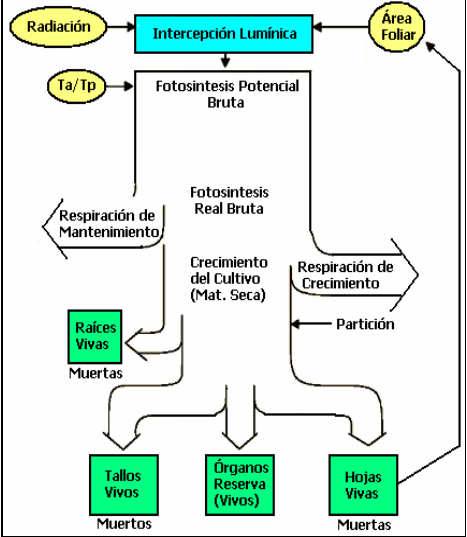
\includegraphics[scale=0.8]{Images/proceso_de_crecimiento_del_cultivo_wofost.png}
	\caption{Procesos del crecimiento del cultivo en WOFOST \parencite{sebem2005aportaciones}}
	\label{fig:img_3}
\end{figure}

La materia seca producida en cada uno de los órganos se calcula en función de la total, aplicando factores que son función del estadio de desarrollo fenológico del cultivo. La curva de crecimiento del cultivo se obtiene integrando el incremento diario de materia seca, para cada uno de los distintos órganos.\\

Los procesos que son simulados en el sistema pueden reagruparse en:

\begin{enumerate}
	\item Simulación del desarrollo fenológico del cultivo. En todo sistema de simulación es esencial determinar los distintos estados fenológicos de la planta, pues, dependiendo de éstos, los procesos fisiológicos y morfológicos son distintos. El más importante es el cambio entre estado vegetativo y reproductor, pues determina la transformación más significativa de reparto de la materia seca en los distintos órganos. Un cultivo pasar por sucesivos estadios fenológicos, la duración dependerá de la tasa de desarrollo. Los principales estadios fenológicos en cultivos anuales son:
	\begin{itemize}
		\item Fecha de siembra. Puede ser conocida o en su defecto calculada por el modelo. 
		\item Nascencia. Viene caracterizada por la aparición de la parte aérea del cultivo aunque lo normal es que la simulación comience en la nascencia, si se quiere proceder a la simulación desde la fecha de siembra, la fecha de nascencia puede calcularse mediante la suma de temperaturas efectivas (temperaturas comprendidas entre dos límites entre los cuales tienen lugar los procesos fenológicos) a partir de la fecha de siembra.
		\item Floración. Es la etapa en que las glumillas de la flor empiezan a separarse.
		\item Maduración. Se produce cuando los órganos de reserva han alcanzado una composición adecuada para su consumo y conservación. 
	\end{itemize}
	La duración de los distintos estadios es función de la tasa de desarrollo. En el modelo, la tasa de desarrollo antes de la floración está controlada por la temperatura y la longitud del día mientras que después de la floración únicamente está regulada por la temperatura. Temperaturas más altas acortan los periodos de crecimiento ya que la tasa de desarrollo es mayor.
	
	En WOFOST la fenología se describe mediante una variable de estado sin dimensión (D); para la mayoría de los cultivos anuales se considera 0 en la emergencia, 1 en la floración y 2 en la madurez. 
	
	Para determinar el efecto de la temperatura en el estado de desarrollo se emplea el concepto de tiempo termal, definido como la suma de temperaturas o suma de calor. El tiempo termal es la integración en el tiempo de temperaturas diarias efectivas después de la emergencia. La temperatura efectiva es la diferencia entre la temperatura media diaria y una temperatura base por debajo de la cual se considera que no hay desarrollo, esta temperatura efectiva no puede ser negativa ni superior a un máximo incremento diario. El estado fenológico se calcula dividiendo el tiempo termal requerido para pasar de un estado de desarrollo al siguiente. Para calcular el tiempo entre la siembra y la emergencia del cultivo WOFOST utiliza otras variables de tiempo termales.
	
	En algunos cultivos el desarrollo fenológico se ve influido también por el fotoperíodo. Este fenómeno es considerado en WOFOST como un factor de reducción (valor entre 0 y 1) para la tasa de desarrollo hasta floración basado en un fotoperíodo óptimo y crítico.
	
	El estado de desarrollo determina, entre otras cosas, la partición de los asimilados entre los distintos órganos (hojas, tallos, raíces y órganos de reserva). Después de la germinación la mayoría de los asimilados se convierten en tejido foliar o radicular y posteriormente en tallo. La partición en tejido radicular disminuye gradualmente llegando a cero cuando el desarrollo es 1 (floración). A partir de la floración los órganos de reserva reciben la mayor parte de los asimilados disponibles. 
	
	En los cálculos, se asigna primero una fracción de los asimilados a las raíces, el resto se divide entre los órganos por encima del suelo. Para iniciar la simulación se debe conocer el peso seco y el índice de área foliar en la emergencia. Desde el principio del crecimiento del cultivo, la reserva de asimilados en las hojas determina el incremento del índice foliar, calculado multiplicando el peso de la materia seca de las hojas por el área foliar específica. Sin embargo la expansión del área foliar puede verse limitada por el incremento máximo diario en el índice de área foliar que depende de la temperatura. El aumento del área foliar conlleva una mayor intercepción de la luz y, por tanto, una mayor tasa de crecimiento potencial. Esto se traduce en un crecimiento exponencial que dura hasta que toda la luz es interceptada (LAI>=3). Seguidamente el crecimiento es constante hasta que el área foliar y su capacidad de fotosíntesis disminuye debido a la senescencia del cultivo. 
	
	\item  La producción diaria de materia seca. Se estima mediante el cálculo de la tasa bruta de asimilación de $ CO_2 $ total diaria y la asimilación bruta de $ CO_2 $ total instantánea con base diaria. La primera puede ser calculada integrando la asimilación de $ CO_2 $ bruta total instantánea con base diaria. La asimilación se origina por la luz interceptada, de modo que esta integración sólo es necesaria si se produce asimilación instantánea, por ejemplo, si no existe superficie foliar no hay luz interceptada y no hay fotosíntesis.
	
	\item La asimilación real de $ CO_2 $. Se obtiene a partir de la asimilación bruta de $ CO_2 $ al tener en consideración el gasto de $ CO_2 $ debido principalmente a la respiración de mantenimiento, respiración de crecimiento y a reparto de la materia seca. 
	
	Parte de los hidratos de carbono producidos se respiran para mantener las estructuras, este proceso puede consumir del 15 al 30\% de los carbohidratos producidos durante el ciclo del cultivo con lo que resulta importante cuantificar con precisión este proceso. La planta también consume los compuestos de carbono sintetizados durante la fotosíntesis en su propio crecimiento. Los asimilados se reparten en la planta según el estado fenológico y los distintos órganos, la tasa de la materia seca total del cultivo puede considerarse como:
	\begin{align*}
		&\Delta W = C_e R_g\\
		&\text{donde: } \\
		&\Delta W  \Rightarrow \text{ tasa de crecimiento de la materia seca total del cultivo [$ kg \; ha^{-1} \; d^{-1} $] } \\
		&C_e  \Rightarrow \text{ factor de eficiencia de la conversión de asimilados [$ kg \; kg^{-1} $] } \\
		&R_g \Rightarrow \text{tasa de respiración de crecimiento [$ kg \; ha^{-1} \; d^{-1} $] } \\
		&\text{donde $ C_e $ se define como: } \\ 
		&C_e = \frac{1}{\sum_{i=1}^{i=2}\frac{pc_i}{C_{e,i}}(1-pc_{rt})+\frac{pc_{rt}}{C_{e,rt}} } \\
		&\text{donde: } \\
		& C_{e,i}  \Rightarrow \text{ factor de eficiencia de conversión de los asimilados de un órgano específico [$ kg \; kg^{-1} $] } \\
		& pc_i  \Rightarrow \text{ factor de partición del órgano $ i $ [$ kg \; kg^{-1} $] } \\
		& i \Rightarrow \text{ hojas (lv), órganos de reserva(so), tallos (st) } \\
		& rt \Rightarrow \text{raíces}
	\end{align*}
	
	Para poder hacer girar el modelo son necesarios, para cada cultivo, una numerosa seria de parámetros que se determinan empíricamente, por ejemplo para estimar la fecha de emergencia es necesario conocer la suma de temperaturas medias diarias (TSUMEN) que se considera estiman el tiempo transcurrido entre la siembra y la nascencia del cultivo, estas temperaturas medias deben superar una temperatura base (TBASEM) y sin sobrepasar un incremento máximo diario (TEFFMX). 
	
\end{enumerate}


\subsection{Sub-modelo de Agua en el Suelo \parencite{sebem2005aportaciones}}

Es importante para un modelo de simulación tener en cuenta el balance hídrico para conocer si un cultivo está sujeto a estrés. Su objetivo será calcular diariamente la cantidad real de agua del suelo para que determinar el agua disponible para el cultivo y su transpiración. La simulación de las variables biológicas (rendimiento de los órganos de almacenamiento y biomasa total) se ha realizado para condiciones sin limitación de agua y considerándola factor limitante. 

Para el cálculo de los flujos de agua se requiere conocer los parámetros de pluviosidad, superficie de almacenamiento, superficie de escorrentía, evaporación de la superficie del suelo, transpiración del cultivo, percolación de la zona de enraizamiento a horizontes más profundos y ascensión capilar a la zona de raíces. 

El contenido real del agua en el suelo puede estimarse mediante la ecuación:
\begin{align*}
	&\theta_t = \frac{IN_{up}+(IN_{low}-T_a)}{RD}\Delta t \\
	&\text{donde: } \\
	&IN_{up}=P+I_e-E_s+SS_t/\Delta t - SR \\
	&IN_{low}=CR-Perc \\
	&\text{donde: } \\
	&\theta_t  \Rightarrow \text{ contenido en agua real de la zona de las raíces en el intervalo de tiempo [$ cm^3 \; cm^{-3} $] } \\
	&IN_{up} \Rightarrow \text{ tasa de afluencia neta a través del límite superior de la zona radicular [$ cm \; d^{-1} $]} \\
	&IN_{low} \Rightarrow \text{ tasa de afluencia neta a través del límite inferior de la zona radicular [$ cm \; d^{-1} $]} \\
	&T_a \Rightarrow \text{ tasa de transpiración real del cultivo [$ cm \; d^{-1} $]} \\
	&RD \Rightarrow \text{ profundidad real de enraizamiento  [$ cm $]} \\
	&P \Rightarrow \text{ intensidad de la precipitación  [$ cm \; d^{-1} $]} \\
	&I_e \Rightarrow \text{ irrigación diaria efectiva  [$ cm \; d^{-1} $]} \\
	&E_s \Rightarrow \text{ tasa de evaporación del suelo [$ cm \; d^{-1} $]} \\
	&SS_t \Rightarrow \text{ superficie de almacenamiento [$ cm $]} \\
	&SR \Rightarrow \text{ tasa de escorrentía [$ cm \; d^{-1} $]} \\
	&SR \Rightarrow \text{ tasa de ascenso capilar [$ cm \; d^{-1} $]} \\
	&Perc \Rightarrow \text{ tasa de percolación [$ cm \; d^{-1} $]} \\
	&\delta t \Rightarrow \text{ intervalo de tiempo [$ d $]} \\
	&Z_t \Rightarrow \text{ profundidad de la capa freática [$ cm $]} \\
\end{align*}

Los procesos que afectan directamente al contenido en agua del suelo radicular (figura \ref{fig:img_4}) son:
\begin{enumerate}
	\item Infiltración : paso del agua de la superficie del suelo a la zona radicular.
	\item Evaporación : pérdida de agua del suelo a la atmósfera.
	\item Transpiración : pérdida de agua.
	\item Percolación : transporte hacia abajo del agua de la zona radicular a la zona inferior a ésta.
	\item Ascensión capilar : transporte hacia la zona radicular.
\end{enumerate}

\begin{figure}[!h]
	\centering
	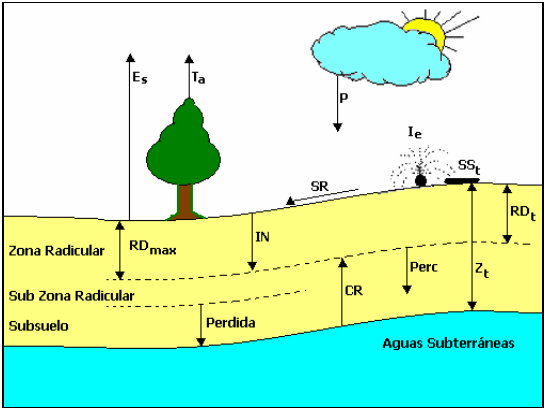
\includegraphics[scale=0.8]{Images/representacion_esquematica_de_los_componentes_del_balance_del_agua_suelo.png}
	\caption{- Representación esquemática de los componentes del balance de agua del suelo. \parencite{sebem2005aportaciones}}
	\label{fig:img_4}
\end{figure}

El contenido en agua de la zona radicular se obtiene a partir del cálculo diario del balance hídrico. En WOFOST se distinguen tres diferentes submodelos de agua en el suelo. Aunque WOFOST admite tres tipos de cálculos distintos del balance hídrico, el WOFOST de CGMS sólo considera los dos primeros sub-modelos, el tercero no es operativo por no disponer al pF del suelo.
\begin{enumerate}
	\item Cálculo del balance hídrico del suelo para la producción potencial: El más simple de los balances se aplica para simular la producción potencial. Se considera que la planta crece sin estrés hídrico asumiendo que el suelo está permanentemente a capacidad de campo, de modo que:
	\begin{align*}
		&\theta_t=\theta_{fc} \\
		&\text{donde: } \\
		&\theta_t  \Rightarrow \text{ contenido real del agua del suelo [$ cm^3 \; cm^{-3} $] } \\
		&\theta_{fc}  \Rightarrow \text{ contenido a capacidad del campo [$ cm^3 |; cm^{-3} $] } \\
	\end{align*}
	En los cálculos no se tienen en cuenta la precipitación, irrigación, ascensión capilar y el drenaje, aunque estos procesos puedan ocurrir. Los únicos dos procesos que se consideran son la transpiración del cultivo y evaporación del suelo.
	
	La tasa de evaporación para la mayoría de los cultivos (cultivos sin conductos de aire en las raíces y que no soportan el encharcamiento) se calcula como la tasa de evaporación de la superficie del suelo:
	\begin{align*}
		&E_s=E_{s,max}\frac{\theta_{fc}-\frac{\theta_{wp}}{3}}{\theta_{max}-\frac{\theta_{wp}}{3}} \\
		&\text{donde: } \\
		&E_s  \Rightarrow \text{ tasa de evaporación de la superficie de suelo sombreada [$ cm \; d^{-1} $] } \\
		&E_{s,max}  \Rightarrow \text{ tasa de evaporación máxima de la superficie de suelo sombreada [$ cm \; d^{-1} $] } \\
		&\theta_{wp}  \Rightarrow \text{ contenido en agua en el punto de marchites [$ cm^3 \; cm^{-3} $] } \\
		&\theta_{max}  \Rightarrow \text{ porosidad del suelo [$ cm^3 \; cm^{-3} $] } \\
		&\text{Calculándose la máxima tasa de evaporación de la superficie de suelo sombreado como: } \\
		&E_{s,max}=EO_se^{-k_{gb}LAI} \\
		&\text{donde: } \\
		&EO_s  \Rightarrow \text{ tasa de evaporación potencial de la superficie de un suelo desnudo [$ cm \; d^{-1} $] } \\
		&k_{gb}  \Rightarrow \text{ coeficiente de extinción para la radiación global total [$ - $] } \\
		&LAI  \Rightarrow \text{ índice de área foliar [$ ha \; ha^{-1} $] } \\
	\end{align*}
	\item Cálculo del balance hídrico del suelo cuando no se considera la capa freática: El segundo sub-modelo para la situación de producción con limitaciones de agua se aplica a un suelo que drena libremente, la capa freática es tan profunda que no influye en el contenido de agua de la zona radicular. 
	
	Para la zona de enraizamiento se calcula diariamente la ecuación del balance hídrico. El balance hídrico es impulsado por la precipitación y la evapotranspiración. Los procesos considerados son la infiltración, retención de agua en el suelo, percolación y pérdida de agua por debajo de la zona radicular máxima. El agua puede retenerse en el suelo hasta el contenido de la capacidad de campo. Se distinguen en el suelo tres zonas:
	\begin{enumerate}
		\item zona de enraizamiento, entre la superficie y la profundidad real de las raíces.
		\item zona inferior, entre la profundidad real de enraizamiento y la máxima.
		\item subsuelo, por debajo de la profundidad máxima.
	\end{enumerate}
	\item Cálculo del balance hídrico del suelo cuando se considera la capa freática: El tercer sub-modelo se aplica para calcular la producción con limitación de agua en suelos que tienen la influencia de una capa freática poco profunda en la zona radicular. La diferencia con respecto al segundo submodelo es que la capacidad de retención del agua en el suelo está determinada por la profundidad de la capa freática, es decir, la tasa de percolación.
	
	Aunque las simulaciones se llevan a cabo mediante CGMS también se ha utilizado el modelo de simulación WOFOST 7.1 con la utilidad WCC (WOFOST Control Centre 1.5). WCC facilita la selección de los ficheros correspondientes al clima, cultivos y suelo así como el tratamiento y visualización de los datos resultantes de la simulación. 
	
	Existe la opción de realizar varias simulaciones a la vez (rerun) cambiando algunos de los parámetros con el objeto de estudiar el cambio de las variables simuladas. 
	
	Mediante WOFOST se pueden obtener distintos tipos de resultados: 
	\begin{enumerate}
		\item \textbf{Potenciales}. Producción potencial del cultivo: (IDSEM) Número de días desde la nascencia (d); (DVS) Estado de desarrollo del cultivo (-); (TSUM) Tiempo térmico desde la nascencia (ºC d); (WLV) Peso seco de las hojas vivas (k ha); (WST) Peso seco de las tallos vivas (k ha); (WSO) Peso seco de las órganos de reserva vivos (k ha); (TAGP) Producción total sobre el suelo (órganos vivos y muertos) (k ha); (LAI) Índice de Área Foliar (área foliar/superficie del suelo) (ha/ha); (TRA) Tasa de transpiración (mm/d); (GASS) Tasa de asimilación bruta (mm/d); (MRES) Tasa de respiración de mantenimiento (mm/d); (DMI) Incremento de la tasa de materia seca (k/ha d). 
		\item\textbf{ Con limitación de agua}. Producción con limitación de agua: (WLV) Peso seco de las hojas vivas (k ha); (WST) Peso seco de las tallos vivas (k ha); (WSO) Peso seco de las órganos de reserva vivos (k ha); (TAGP) Producción total sobre el suelo (órganos vivos y muertos) (k ha); (LAI) Índice de Área Foliar (área foliar/superficie del suelo) (ha/ha), (RD) Profundidad de la zona de enraizamiento real (cm); (SM) Contenido de agua en el suelo en la zona de enraizamiento real (cm3 agua/cm3 suelo); (RESRV) Agua del suelo disponible en la zona de enraizamiento potencial (en y por debajo de la zona de enraizamiento real) (cm suelo); (AVAIL) Agua disponible en la zona de enraizamiento real (cm agua) Sólo cuando se simula sin la influencia de agua subterránea); (RAIN) Precipitación total en el período de simulación (mm); (TRA) Tasa de transpiración (mm/d); (EVA(P)) Tasa de evaporación desde el suelo o del agua almacenada en la superficie del suelo (mm/d); (SS) Superficie de almacenamiento (cm agua); (ZT) Profundidad de la capa freática (cm por debajo de la superficie del suelo); (wet) Días caracterizados por un crecimiento reducido debido a la falta de oxígeno (d); (dry) Días caracterizados por un crecimiento reducido debido a la falta de agua (d). 
		\item\textbf{ Con limitación de nutrientes}. Producción con limitación de nutrientes: Este caso no va a ser considerado en los procesos de simulación que van a llevarse a cabo ya que no se dispone de los datos. 
		\item\textbf{ Balance hídrico}. Los resultados de balance hídrico se obtienen tanto para todo el sistema como para la zona radicular. Para todo el sistema los resultados que obtenemos son: (1) Contenido de agua inicial y final y su diferencia (bien para la zona radicular máxima o para los 10 primeros cm cuando consideramos la influencia del agua del suelo); (2) Superficie de almacenamiento de agua inicial y final y su diferencia; (3) Precipitación; (4) Evaporación (del suelo o la superficie de agua) y transpiración (del cultivo); juntos son pérdida de agua a la atmósfera y (5) Agua de escorrentía, percolación al agua del terreno y pérdida de agua debida al drenaje (cuando hay agua freática).
		
		Los resultados del balance hídrico en la zona radicular comprende los siguientes datos: (1) Contenido de agua inicial y final y su diferencia en la zona radicular; (2) Infiltración a la zona radicular (ejemplo, precipitación menos escorrentía); (3) Evaporación (del suelo) y transpiración (del cultivo); (4) Incremento del agua disponible debido al crecimiento radicular; (5) Percolación al agua del suelo y (6) Aumento de la capilaridad (cuando existe agua freática).
		
		\item Resultados resumidos: WCC resume en un fichero las variables de salida para los distintos años, así como los datos estadísticos (media, desviación típica y coeficiente de variación) de todos los años.
	\end{enumerate}
\end{enumerate}


















